\documentclass[addpoints,12pt]{exam}
\usepackage{amsmath,amsthm,amssymb}
\linespread{1.05}
\usepackage{hyperref}
\usepackage[top=0.5in,bottom=1in,left=1in,right=1in]{geometry}
\usepackage[linesnumbered,ruled]{algorithm2e}
\usepackage[dvipsnames]{xcolor}
\usepackage{tikz}
\usepackage[framemethod=TikZ]{mdframed}

\usepackage{graphicx}
\graphicspath{ {./images/} }

\printanswers
\marksnotpoints

\pointformat{\textcolor{Maroon}{(\thepoints)}}
\qformat{\textcolor{Maroon}{\textbf{Problem~\thequestion}} \hfill \textcolor{Maroon}{\textbf{\totalpoints~\points}}}


\newcommand{\course}{{\large CS6170: \textsc{Randomized} \textsc{Algorithms}}}
\newcommand{\pset}[1]{{\large \textsc{Problem} \textsc{Set} \##1}}
\newcommand{\due}[1]{{\textsc{Due}: #1}}
\newcommand{\name}[1]{\textsc{Name}: \textcolor{Blue}{#1}}
\newcommand{\rno}[1]{\textsc{Roll} \textsc{No}: \textcolor{Blue}{#1}}
\pagestyle{plain}

\newcommand\geqques{\stackrel{\mathclap{\normalfont\mbox{?}}}{>}}

\begin{document}
	
	\hrule height 2pt
	\vspace{2mm}
	{\centering \course \par}
	\vspace{1mm}
	{\centering \pset{1}\par}
	\vspace{1mm}
	\noindent \name{Akash Roy} \\
	\rno{CS22M007}\hfill \due{August 22, 23:59}
	\vspace{2mm}
	\hrule height 2pt
	\vspace{2mm}
	
	\begin{questions}
		
		\question [3] Consider the following variation of Karger's algorithm, wherein we sample two vertices independently and uniformly at random and contract them to create a supernode (instead of sampling an edge at random). Show that there exist graphs where the probability that this algorithm outputs the mincut is exponentially small.
		\begin{solution}
			Discussed with Ramaswamy Kandaswamy. The approach may not match with him. \\

                We've analyzed with various special graphs, including bipartite, and line graphs but those did not yield any good results. Finally, we can conclude that graphs connected with one edge with both sides being a complete sub-graph (clique) has an exponentially small min-cut survival rate.

                Let's consider one graph $G$ that has $2n$ vertices and there are 2 complete subgraphs of size $n$ connected by one edge $e$. This edge $e$ is the unique min cut of the graph $G$.

                Probability of the cut surviving is that we don't sample 2 vertices across the 2 complete sub graph. The cut will only survive if we choose 2 vertices either from left complete graph or from right complete graph. So that would be for the first iteration:
                $$
                \Pr(\text{Min cut is survived in the first go}) = \frac{\binom{n}{2} + \binom{n}{2}}{\binom{2n}{2}}
                $$

                For any general i step of the iteration let's say there is $x$ nodes in the left subgraph and y $nodes$ in the right subgraph. For this step of the algorithm $x + y = n - i + 1$.

                For this step the probability that we don't destroy the cut is 

                \begin{align*}
                    \Pr(E_i | E_1 \cap E_2 \cap E_3 \cap ... \cap E_K) &= \frac{\binom{x}{2} + \binom{y}{2}}{\binom{x+y}{2}}\\
                    &= 1 - \left(\frac{2xy}{(x+y)^2 + x + y}\right)
                \end{align*}

                As $x + y = n - i + 1$ we can say that for any $i < \frac{n}{j}$ where $j \in \mathbb{N} \setminus \{1\}$ we can bound $x$ and $y$ as $x \geq \frac{n}{j}$ and $y \geq \frac{n}{j}$

                So now 
                \begin{align*}
                    \Pr(E_i | E_1 \cap E_2 \cap E_3 \cap ... \cap E_K) &= 1 - \frac{2 (\frac{n}{j}) * \frac{n}{j}}{n^2}\\
                    &= 1 - \frac{2}{j^2}
                \end{align*}

                Now the probability of surviving a cut edge till $n-2$ step is $\leq$ probability of surviving the cut edge till $\frac{n}{j}$.

                So $\Pr(\text{Cut survives } n - 2 \text{ steps}) \leq \Pr(\text{Cut survives } \frac{n}{j} \text{steps})$

                Now say $\Pr(\text{Cut survives at step i}) = \Pr(E_i)$
                \begin{align*}
                    \Pr(\text{Cut survives } n - 2 \text{ steps}) &\leq \Pr(\text{Cut survives } \frac{n}{j} \text{steps})\\
                    &= \Pr(E_1) * \Pr(E_2) ... \Pr(E_{n -2}))\\
                    &\leq \Pr(E_1) * \Pr(E_2) ... \Pr(E_{\frac{n}{j}})\\
                    &= (1 - \frac{2}{j^2})^{\frac{n}{j}}\\
                \end{align*}

                Taking j = 3 as any arbitrary value we'll get the probability as a function of $(\frac{7}{9})^{O(n)}$. This shows the exponentially low probability for the survival of the cut set.
		\end{solution}
		
		\question[5] Consider the following game: We start with one black ball and one white ball in a bin. We repeatedly do the following until there are $n$ balls in the bin: we choose a ball uniformly at random, put the ball back in the bin together with another ball of the same color. Show that the number of white balls is equally likely to be any number between $1$ and $n-1$.
		\begin{solution} \textbf{Discussed with Ramasamy Kandasamy}\\
			Our starting point is a box with a black and a white ball. We choose balls uniformly at random from the box and then put that color of the ball along with the original ball back into the box.

            Our game's termination point is when we reach total of $n$ balls in a box. So let's start our game with one white and one black ball in the box. Here say this is iteration \#1. For our iteration one we have 2 choices, we can uniformly at random take a black ball or take a white ball. If we have taken a white ball, at the start of the second iteration number of balls that is white is 2 or if we've taken a black ball, number of white balls to be found is 1.

            Now for the third iteration, we have 2 choices of choosing a black ball and one choice of choosing a white ball. Let's draw a tree based on the choices.

            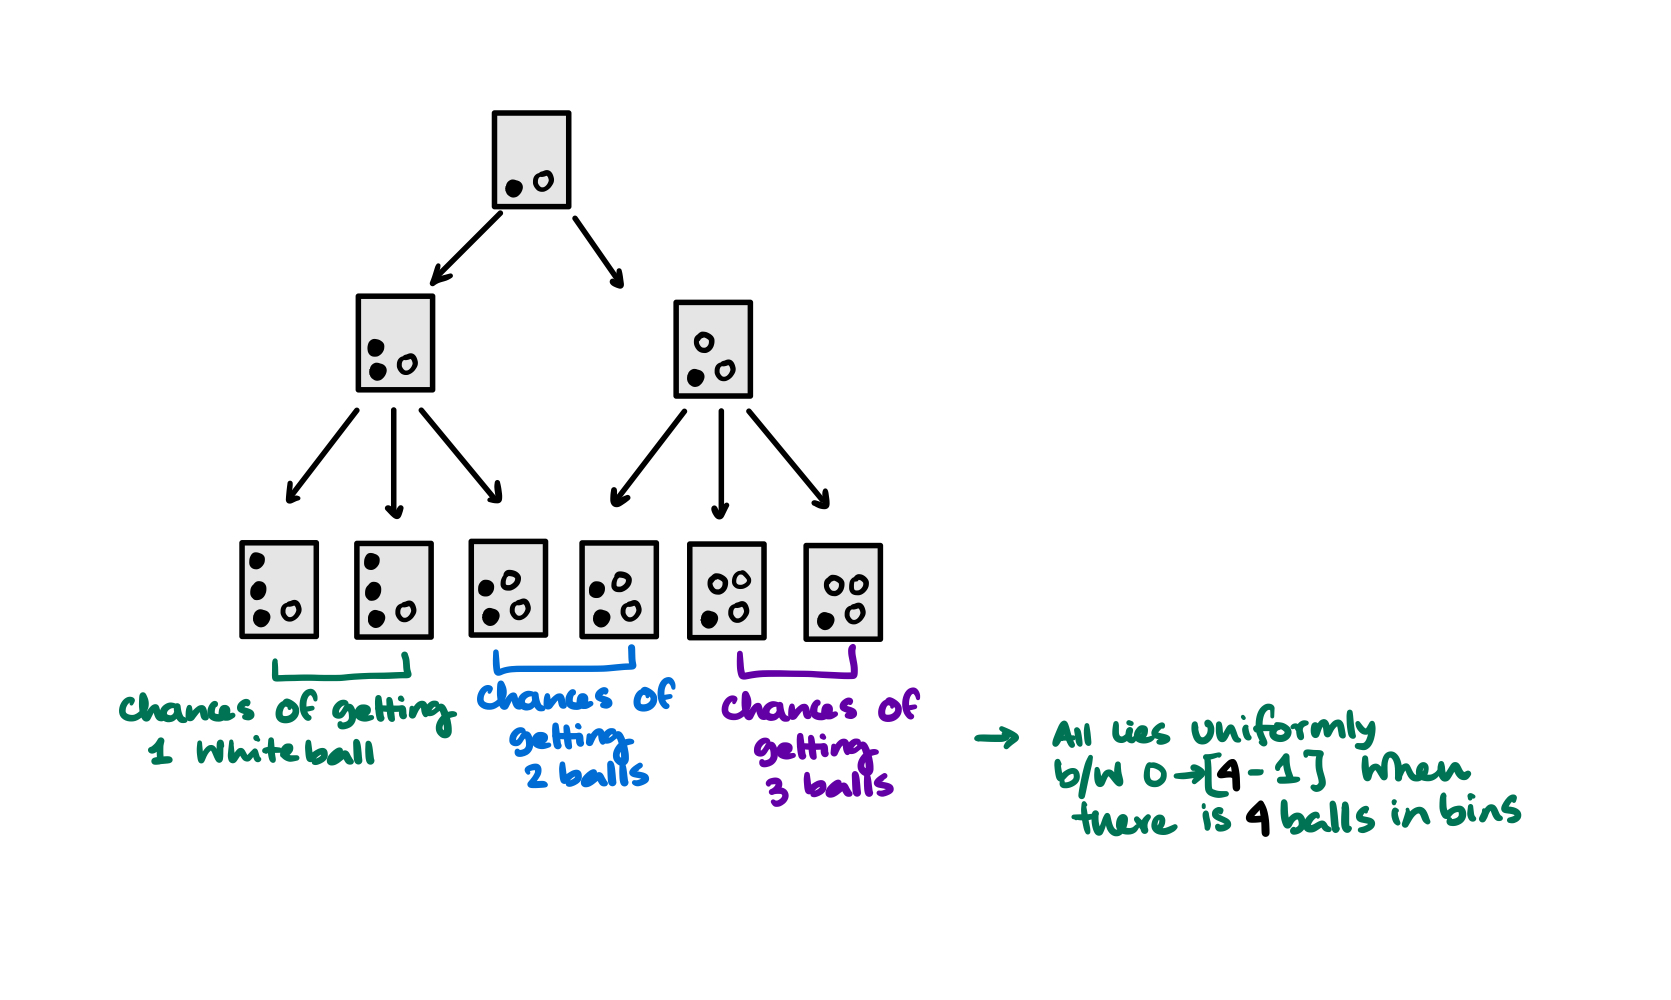
\includegraphics[scale=0.27]{ballsnbins}

            So for our induction base case till box having a number of balls $= 4$ we have a uniform distribution on the number of white balls in a box from $1 \to (4-1)$ all being equal to $2$.

            Our induction hypothesis is the following that our assumption is true when there are $i$ many balls in the bin. If we can show our assumption is true for $i+1$ many balls in the bin then our induction hypothesis holds true for $n \in \mathbb{N}$. I am defining $i$ many balls is at the $i^{th}$ level. So our \textbf{probability tree} starts at level $2$. I'm also defining \textbf{probability tree} as the tree generated by the choices at each node of the tree. Each node of the tree is a possible configuration of the box during a random choice of a ball. Any game is a path from the root of the tree to a leaf of the tree.

            So our hypothesis is true for $i$ many balls in the bin. Now there can be from $1 \to i-1$ many white balls at this level each with same probability out of all possible orderings of balls at level $i$. So base case is verified. Now we make a hypothesis and prove it through induction.
            
            For example, the figure up above shows all the possible combinations of black and white balls when there are 4 balls in the box. Chances of getting white ball $= k \in \{1,2,3\}$ are $2$ out of all possible orderings at the level. If we analyze for one more level $i = 4$ we see that for each $k \in \{1,2,3,4\}$ chances of getting k many balls is $6$ out of all possible ordering at this level.

            Going to the next level (at $i+1$) from this level ($i$) we'll analyze what is going to happen. Some observations from the probability tree are following

            \begin{itemize}
                \item At level 2 (first level, a level $i$ has $i$ many balls in them according to my definition) number of box configurations having $1$ ball is $1! = 1$, at level 3 number of box configurations having $1 \to (3-1)$ white ball is $1! * 2 = 2! = 2$, at level 4 number of box configurations having $1 \to 4$ white ball is $2! * 3 = 3! = 6$, and similarly this is verifiably true for level 5 also. At level 4 there are 4! boxes with only one white ball.
                \item This can be generalized also, let's take level $i$ and from our induction hypothesis let's say there is $(i-2)!$ many configurations of boxes where we can find 1 white ball, there is $(i-2)!$ many configurations of boxes where we can find 2 white balls, ... and so on till $i - 1$ many white balls.
                
            \end{itemize}

            Now let's analyze this case. Number of configurations where there is 1 white balls at level $i$ = $(i-2)!$ through induction hypothesis. So Number of configurations where there is 1 white ball in the next level $(i + 1)^{th}$ level = $(i-2)! * (i-1)$ (For each of the $(i-2)!$ cases of one white ball configurations in level $i$ we could choose one black ball $i-1$ times to make one white ball configuration in the level $i+1$).

            Similarly number of configurations with 2 white balls at level $i = (i-2)!$. Now Let's look at the same for level $i+1^{th}$. So all 2 ball configurations will come from 2 ball configurations from the last level and one 1-ball box configuration from the last level (through the choice of 1 white ball). So the number of possible configurations will be $(i-2)! * (i-2) + 1$

            Similarly number of configurations with 3 white balls at level $i = (i-2)!$. The number of configurations with 3 balls at level $i+1$ will be the following

            For each possible configurations of 3 white balls in the $i^{th}$ level * $(i-3)$ (i - 3 many black balls replaced would result in 3 white ball configurations) + $(2) * (i - 3)$ (2 white ball replaced in the last level also makes 3 white ball configuration at this level) $= (i-2)! * (i-3) + (i-2)! * 2 = (i-2)! * (i - 1) = (i-1)!$.

            So for any general $j \text{ many white balls } \in \{1, 2, ..., 3^{i + 1}\}$ at level $i + 1$ of the probability tree, number of box configurations with $j$ many white balls is $(i-2)! * (i-j) + (i-2)! * (j-1) = (i-2)! *(i-j + (j - 1)) = (i-2)! * (i-1) = (i-1)!$.

            So our hypothesis holds true for level $i+1$ as well. So we can say for any $n \in \mathbb{N}$ our assumption holds true.

            So for any n size box probability of getting $j$ white balls from box is same / equally likely for any $j \in \{1,2,3,4, ..., n - 1\}$.
            
		\end{solution}
	
		\question[5] Consider a complete rooted $3$-ary tree of height $h$ - every leaf in this tree is at a depth $h$ from the root. Each leaf has a boolean truth value associated with it. The value of an internal node is the majority of the values of its child nodes. Consider the following scheme for evaluating the value of the root node: Randomly choose two child nodes and recursively evaluate them. If they have the same value, then return that value. Else, evaluate the third child recursively and find the majority. Show that the number of truth values of the leaf nodes read by this algorithm is at most $n^{0.9}$, where $n = 3^h$.
		\begin{solution} \textbf{Discussed with Ramasamy Kandasamy}\\
			I've used induction to prove this statement. Let's take a look for the base case how many lookups we are doing?

            Let's say our tree has one root node and 3 children. The values for those children can be $\{000,001,010,011, 100,101,110,111\}$. For values $\{000,111\}$ there can be at most 2 lookups. For any case other than this let's take a look

            For cases $\{001,010,011, 100,101,110\}$ there is a chance that we look at same value for both child so there would be 2 lookups other wise there would be 3 lookups. For example $011$ if we check 1 and 1 then the lookup is 2 and if we look 0 and 1 then our lookup becomes 3. So we could have looked at $\{0, 1(\text{1st one})\}$ or $\{0, 1(\text{second one})\}$ or $\{1(\text{1st one}), 1(\text{second one})\}$. So with probability $\frac{1}{3}$ we lookup 2 times for these 6 cases and with probability $\frac{2}{3}$ we lookup 3 times for these 6 cases $\{001,010,011, 100,101,110\}$.

            So our expected lookup in the base case become
            \begin{align}
                \mathbb{E}(x) &= \frac{2}{8} * 2 + \frac{6}{8} \left[\frac{1}{3}* 2 + \frac{2}{3} * 3\right]\\
                &=2.495\\
                &\leq (3^1)^{0.9} = 2.68
            \end{align}

            So the statement that at any level expected number of lookup at the leaf is at most $3^{0.9}$.

            In my induction base case, it is to be noted that I'm taking levels i = 0 for the leaf because there is no lookup and level 1 is the root. So for the general case our leaves are at $0$ and the root node is at level/height $n$. The words level and height are used synonymously.

            So let's say for our induction hypothesis the statement is true for level $i - 1$. Using this statement if we can show that our statement also holds good for level $i$ then our induction hypothesis is correct for any $n \in \mathbb{N}$.

            Let's consider some random variables $X_i$ for each node in level $i$ indicating the number of lookup from the leafs and for each 3 children of $X_i$ let's take random variables $Y_{i, 1}, Y_{i, 2} \:\&\: Y_{i, 3}$.

            We should be finding that $\displaystyle\sum_{i=0}^{3^{i}} \mathbb{E}(X_i) \leq (3^i)^{0.9}$, then our induction hypothesis becomes true.

            Let's look at one individual node $i$ and let's calculate $\mathbb{E}(X_i)$

            We saw that for any node with $\frac{1}{2}$ probability we'll look at 2 of it's children and with $\frac{1}{2}$ probability we'll look all three of its children.
            
            \begin{align}
                \mathbb{E}(X_i) &= \frac{1}{2} * \left(\mathbb{E}(Y_{i, 1}) + \mathbb{E}(Y_{i, 3}) \right)+ \frac{1}{2} \left(\mathbb{E}(Y_{i, 1}) + \mathbb{E}(Y_{i, 2}) + \mathbb{E}(Y_{i, 3})\right)
            \end{align}
            When number of lookup is $2$ we could have taken $\{1, 3\}, \{1, 2\}, \{2, 3\}$ with $\frac{1}{3}$ probability equally likely so they are symmetrical and $3 * \frac{1}{3} = 1$, so considering any of $\{1, 3\}, \{1, 2\}, \{2, 3\}$ is sufficient.

            So we are required to find out $\displaystyle\sum_{i=0}^{3^{i}} \mathbb{E}(X_i)$, now assuming our induction hypothesis on level / height $i-1$

            \begin{align}
                \displaystyle\sum_{i=0}^{3^{i}} \mathbb{E}(X_i) &= \frac{1}{2} * (2 * \mathbb{E}(Y)) + \frac{1}{2} * (3 * \mathbb{E}(Y))\\
                &= \frac{2}{2} \left[3^{i-1}\right]^{0.9} + \frac{3}{2} \left[3^{i-1}\right]^{0.9}\\
                &= \frac{5}{2} \left[3^{i-1}\right]^{0.9}\\
                &= \frac{\frac{5}{2}}{3^{0.9}} \left[3^{i}\right]^{0.9}\\
                &= \frac{2.5}{2.6}\left[3^{i}\right]^{0.9}\\
                &\leq \left[3^{i}\right]^{0.9}
            \end{align}

        From (10) we established the fact that for height $i$ expected number of lookup in the leaf is at most $\left(3^{i}\right)^{0.9}$

        So from this I can say for $\forall \:n \in \mathbb{N}$ height 3-ary tree must have expected number of lookup in the algorithm upper bounded by $n^{0.9}$.
            
		\end{solution}
	
		\question[5] We have a function $f:\{0,1\}^n \to \{0,1\}$. For every $x,y \in \{0,1\}^n$, we have $f(x \oplus y) = f(x) \oplus f(y)$ ($x\oplus y$ refers to bitwise-XOR). The only way available to us to evaluate $f$ is using a look-up table for $f$. Unfortunately, an evil adversary has corrupted $1/5$-th of the look-up table entries.
		
		Describe a randomized algorithm, that given an input $z$, outputs the correct value $f(z)$ with probability $>1/2$. The input $z$ could be anything, regardless of what values the adversary has changed. In particular, $z$ might be one of the values that the adversary has changed and we may not know this.
		
		\rotatebox{180}{
			\begin{minipage}{\linewidth}
				\textcolor{gray}{\textbf{Hint:} What can you say about $f(w)$ for a random $w$? Can you relate that randomly chosen $w$ to the input $z$ whose value you want to evaluate?}
		\end{minipage}}
  
		\begin{solution} \textbf{Discussed with Ramasamy Kandasamy}\\
            I design the algorithm in the following way
            \newpage
            \begin{algorithm}[H]
                \SetKwInOut{Input}{Input to the algorithm}
                \SetKwInOut{Output}{Output from algorithm}
                
            	\Input{Z is binary string $\in \{0,1\}^n$}
            	\BlankLine
                X = \{x $\in_r \{0,1\}^n$\} and $|X|$ = K, 1 based indexing is assumed\\
                F(Z) = \{$\phi$\}\\
            	\While{$K \geq$ 1}{
                    Binary String $x$ $\gets$ X[K];\\
                    Binary String  Y $\gets f(x \oplus Z)$ through lookup\\
                    Binary String  FZ $\gets f(Z)$ through lookup\\
                    Compute $Y \oplus FZ$ and add to set F(Z) ;\\
                    $K \gets K - 1$;
            	}
            	\Output{Return Majority of K many $f(Z) \in F(Z)$}
            	\caption{\textsc{Randomized Lookup Service}}
            \end{algorithm}

            \textbf{Analysis of the algorithm:} Let's take one random variable \textbf{$X_i$}.

            \begin{equation}
                X_i=
                \begin{cases}
                  1, & \text{if}\ i^{th} \text{entry on F(Z) is correct}\\
                  0, & \text{otherwise}
                \end{cases}
            \end{equation}

            Our goal is to check whether $\displaystyle\sum X_i > \frac{K}{2}$ with at least $\frac{1}{2}$ probability. If the majority of the $f(z)$ is correct then $\displaystyle\sum X_i > \frac{K}{2}$ then our algorithm outputs correctly for input Z. We are to show in our analysis that this happens with at least $\frac{1}{2}$ probability.

            So let's look at our random variable, it takes 2 values $0$ or $1$, so it is a Bernoulli indicator random variable. This random variable follows a binomial distribution. We know the following for a fact that the probability that X takes value from 0 to K is our sample space.

            \begin{align}
                \displaystyle\sum_{i=0} ^{K}\text{Pr(X = i)} &= 1\\
                \displaystyle\sum_{i=0} ^{K}\text{Pr(X = i)} &= \displaystyle\sum_{i=0} ^{K}\binom{K}{i} * p^i * (1 - p)^{K - i}
            \end{align}

            Here $p$ is the probability of $X_i$ taking value 1, which is probability that entry in $F(Z)$ (output of our algorithm) is correct is $\geq$ (at least) for computation $f(x) \:\&\: f(x \oplus Z)$ both is not corrupted. There can be a chance that $f(x) \:\&\: f(x \oplus Z)$ for randomly chosen $x$ both got corrupted but still some how their $\oplus$ (XOR) returns the correct value. So the probability that entry is correct is at least $f(x) \:\&\: f(x \oplus Z)$ both are correct.

            Mathematically we can write: $\Pr(f(Z) \text{ is computed correctly}) \geq \frac{4}{5} * \frac{4}{5} = 0.64$

            Let's analyze equation (13).

            \begin{align}
                \displaystyle\sum_{i=0} ^{K}\text{Pr(X = i)} &= \displaystyle\sum_{i=0} ^{K}\binom{K}{i} * p^i * (1 - p)^{K - i}\\
                &= \displaystyle\sum_{i=0} ^{\frac{K}{2}}\binom{K}{i} * p^i * (1 - p)^{K - i} + \displaystyle\sum_{i=\frac{K}{2} + 1} ^{K}\binom{K}{i} * p^i * (1 - p)^{K - i}
            \end{align}

            Let's take an entry in the first part of the equation (15) and let's compare it with a counterpart in the second part of the equation. We'll compare the following pairs $(i=0 \:\&\: i=K), (i=1 \:\&\: i=K-1), (i=2 \:\&\: i=K-2) \:\&\: ...$ so on. To be more precise we'll compare the followings $(i=\frac{K}{2} - 1 \:\&\: i=\frac{K}{2} + 1), (i=\frac{K}{2} + 2 \:\&\: i=\frac{K}{2} -2) \:\&\: ... \text{till} (i=\frac{K}{2} - \frac{K}{2} \:\&\: i=\frac{K}{2} + \frac{K}{2})$

            From observation we can say this for any general $g > 0$;

            \begin{align}
                \binom{K}{\frac{K}{2} + g} p^{\frac{K}{2} + g} (1-p)^{K - (\frac{K}{2} + g)} > \binom{K}{\frac{K}{2} - g} p^{\frac{K}{2} - g} (1-p)^{K - (\frac{K}{2} - g)}
            \end{align}

            This comes from the fact that $\binom{K}{\frac{K}{2} + g} = \binom{K}{\frac{K}{2} - g}$ and $p \geq 0.64$. So let's find out

            \begin{align}
                p^{\frac{K}{2} + g} (1-p)^{K - (\frac{K}{2} + g)} &\stackrel{?}{>} p^{\frac{K}{2} - g} (1-p)^{K - (\frac{K}{2} - g)}\\
                \left(\frac{p}{1-p}\right)^{2g} &\stackrel{?}{>} 1
            \end{align}

            As $p > (1-p)$ because $p \geq 0.64$ for a positive $g$, line 18 holds good. So for each entry in the first part of the equation line number (15) is smaller than each entry in the second part. So overall the second part is higher and they both sum to 1, so the second part $$\displaystyle\sum_{i=\frac{K}{2} + 1} ^{K}\binom{K}{i} * p^i * (1 - p)^{K - i} > \frac{1}{2}$$

            So the statement says probability that our random variable $X > \frac{K}{2}$ is at least $\frac{1}{2}$. This means our algorithm selects the correct output with majority voting with a probability of at least $\frac{1}{2}$.

            \textbf{No where in our algorithm we assumed anything about} $K$, \textbf{so K can be any number} $\in \mathbb{N}$. If we take $K = 3$ and take the majority our algorithm still will output the correct result with a probability of at least $\frac{1}{2}$.
            
		\end{solution}
  
		\question You need a new staff assistant, and you have $n$ people to interview. You want to hire the best candidate for the position. When you interview a candidate, you can give them a score, with the highest score being the best and no ties being possible. You interview the candidates one by one. Because of your company’s hiring practices, after you interview the $k^{th}$ candidate, you either offer the candidate the job before the next interview or you forever lose the chance to hire that candidate. Suppose that the candidates are interviewed in a random order, chosen uniformly at random from all $n!$ possible orderings.
		
		We consider the following strategy. First, interview $m$ candidates but reject them all; these candidates give you an idea of how strong the field is. After the $m^{th}$ candidate, hire the first candidate you interview who is better than all of the previous candidates you have interviewed so far.
		
		\begin{parts}
			\part[4] Let $E$ be the event that we hire the best assistant and let $E_i$ be the event that the $i^{th}$ candidate is the best and we hire him. Determine $\Pr[E_i]$ and show that 
			\begin{align*}
				\Pr[E] &= \frac{m}{n} \sum_{j=m+1}^n\frac{1}{j-1}.
			\end{align*}
			\begin{solution} Did \textbf{NOT} discussed with anyone.\\
                Probability of the event $\mathbb{E}$ that we hire the best candidate can be broken into the following set of events.

                \begin{align*}
                    \Pr(\mathbb{E}) = \displaystyle\sum_{i = 1} ^{n} \Pr(\mathbb{E}_i)
                \end{align*}
                Here $\mathbb{E}_i$ is the event that the best candidate is at location $i$ in the interview queue and we hire him.

                In our strategy we reject the first $m$ candidates so $\displaystyle\sum_{i = 1} ^{m} \Pr(\mathbb{E}_i) = 0$

                We are required to analyze the chances of selecting and hiring the best candidate from $(m+1) \to n$. So let's take any general $g \text{ s.t } m+g \leq n$ and analyze $\Pr(\mathbb{E}_{m + g})$. I'll take $m+g = j$ to match my result with the question. 
                
                The probability of hiring the best guy from location $m+g$ is equal to the probability of the best guy sitting at that location $m+g$ ($\Pr = \frac{1}{n}$) in the interview queue \textbf{AND} from location, $m+1$ till $m+g - 1$ rank of candidates is less than the highest among the first $m$ candidates (say $m_x$) \textbf{AND} we hire him (with probability = 1).

                So in order to successfully hire the best guy from the $m+g = j^{th}$ location no better candidates in the interview queue should be present than the first $m$ candidates between location $m+1 \to j-1$.
                
                \begin{align*}
                    \Pr(\mathbb{E}_{m + g}) &= \Pr(\forall x \in \text{Queue}[m+1 \to m+g], \text{rank}(x) < rank(m_x)) * \frac{1}{n}
                \end{align*}

                This is hard to analyse so, the equivalent thing to say is to say the following statement.

                Starting from $1 \to m$ the best guy among $1 \to j-1$ should be inside there. Because if the best guy from $1 \to j-1$ (this is not the best guy among all the candidates because the global best candidate should be at the $j^{th}$ location) is outside $1 \to m$ then we have to hire this guy instead of the global best candidate sitting at location $j$ in the interview queue.

                So we should calculate what is the probability that the best guy from $1 \to j-1$ is in location $1 \to m$.

                \begin{itemize}
                    \item So best guy till $j-1$ is at location 1 $= \frac{1}{j-1}$
                    \item Best guy till $j-1$ is at location 2 $= \frac{1}{j-1}$
                    \item Best guy till $j-1$ is at location 3 $= \frac{1}{j-1}$
                    \item ... and so on.
                \end{itemize}

                So the best guy till $1 \to j -1$ is in the first $m$ slots of the interview queue is 
                
                $$\displaystyle\sum_{0} ^{m} \frac{1}{j-1} = \frac{m}{j-1}$$

                \begin{align*}
                    \Pr(\mathbb{E}) &= \displaystyle\sum_{j = m+1} ^{n} \Pr(\mathbb{E}_{i})\\
                    &= \displaystyle\sum_{j = m+1} ^{n} \frac{m}{j-1} * \frac{1}{n} * 1\\
                    &= \frac{m}{n} \displaystyle\sum_{j = m+1} ^{n} \frac{1}{j-1}
                \end{align*}
                
			\end{solution}
			\part[3] Using the bounds on harmonic sums we discussed in class, show that the probability is maximized for $m = n/e$, and hence conclude that for this value of $m$, we have
			$$\Pr[E] \geq 1/e.$$
			\begin{solution} Did \textbf{NOT} discussed with anyone.\\
				I'll approximate this quantity from the harmonic sum formula

                \begin{align*}
                    \displaystyle\sum_{j = m+1} ^{n} \frac{1}{j-1} &= \displaystyle\sum_{j = 2} ^{n} \frac{1}{j-1} - \displaystyle\sum_{j = 2} ^{m} \frac{1}{j-1}\\
                    &\approx \ln(n) - \ln(m)\\
                    \therefore \Pr[E] &\thickapprox \frac{m}{n} \left(\ln(n) - \ln(m)\right)
                \end{align*}

                So we need to maximize this so let's take a derivative with respect to $m$ and equate it to $0$.

                \begin{align*}
                    \frac{d}{dm} \left[\frac{m}{n} \left(\ln(n) - \ln(m)\right)\right] &= \frac{d}{dm} \left[\frac{m}{n} \ln\left(\frac{n}{m}\right)\right]\\
                    &= \frac{d}{dm} \left[ m \frac{\ln(n)}{n} - m \frac{\ln m}{n}\right]\\
                    &= \left[ \frac{d}{dm} m \frac{\ln(n)}{n} - \frac{d}{dm} m \frac{\ln m}{n}\right]\\
                    &= \left[\frac{\ln(n)}{n} - \left(\frac{\ln m}{n} + \frac{m}{n} * \frac{1}{m}\right) \right]\\
                    &= \frac{\ln n}{n} - \frac{\ln m}{n} - \frac{1}{n}\\
                    \frac{\ln n}{n} - \frac{\ln m}{n} - \frac{1}{n} &= 0\\
                    \ln m &= \ln n - 1\\
                    m &= e^{\ln n - 1}
                \end{align*}

                So the probabilty is maximized at $m = e^{\ln n - 1} = e^{\ln n - \ln e} = \frac{n}{e}$.

                Now for that value of $m$ our probability becomes
                
                \begin{align*}
                    \Pr(\mathbb{E}) &\geq \left[\frac{m}{n} \ln\left(\frac{n}{m}\right)\right]\\
                    &\geq \left[\frac{\frac{n}{e}}{n} \ln\left(\frac{n}{\frac{n}{e}}\right)\right]\\
                    &= \frac{1}{e}
                \end{align*}
                
			\end{solution}
		\end{parts}
	
		\question Suppose we flip a coin $n$ times to obtain a sequence of flips $X_1, X_2, \ldots, X_n$. A \emph{streak} of flips is a consecutive subsequence of flips that are all same (either all heads or all tails).
		\begin{parts}
			\part[2] Let $n$ be a power of $2$. Show that the expected number of streaks of length $\log_2 n + 1$  is $1 - o(1)$.
			\begin{solution} Discussed with Krishna (ee19d410@smail.iitm.ac.in) \\
				Let's take any $K \in \mathbb{N}$ as a length of the streak. For streak of size $K$ tossed coin $X_j, X_{j+1}, ..., X_{j + k -1}$ should either be all head or all tails.

                Let's take one random variable $Z_i$ such that 
                
                \begin{equation}
                Z_i=
                \begin{cases}
                  1, & \text{if}\ X_j \to X_{j + K - 1} \text{ are all head or all tails}\\
                  0, & \text{otherwise}
                \end{cases}
                \end{equation}

                Now expected value of $Z_i$ for any $i$ would be $\mathbb{E}(Z_i) = \Pr(Z_i = 1) = \frac{1}{2^K} + \frac{1}{2^K} = \frac{2}{2^K}$

                Now $\displaystyle\sum_{1} ^{n - (k -1)} \frac{2}{2^K}$ is the expected number of streaks of size K.

                \begin{align*}
                    \displaystyle\sum_{1} ^{n - (k -1)} \frac{2}{2^K} = (n - (k - 1)) \left[\frac{2}{2^K}\right]
                \end{align*}

                Setting $K = \lg n + 1$ we get

                \begin{align*}
                    \displaystyle\sum_{1} ^{n - (k -1)} \frac{2}{2^K} &= (n - (k - 1)) \left[\frac{2}{2^K}\right]\\
                    &= (n - (\lg n + 1 - 1)) \left[\frac{2}{2^{\lg n + 1}}\right]\\
                    &= (n - \lg n) \left[\frac{2}{2^{\lg n + \lg 2}}\right]\\
                    &= (n - \lg n) \left[\frac{2}{2^{\lg 2n}}\right]\\
                    &= (n - \lg n) \left[\frac{2}{2n}\right]\\
                    &= 1 - \frac{\lg n}{n}
                \end{align*}

                For $n_0 > 2$ $\forall n > n_0$ and $c = 1$ $\frac{\lg n}{n}$ is $o(1)$. So we can say that the expected number of streaks of length $\lg n + 1$ is $1 - o(1)$.
            
			\end{solution}
			\part[3] Show that, for sufficiently large $n$, the probability that there is no streak of length at least $\lfloor \log_2 n - \log_2\log_2 n\rfloor$ is less than $1/n$.
			
			\rotatebox{180}{
				\begin{minipage}{\linewidth}
					\textcolor{gray}{\textbf{Hint:} Break the sequence of flips into disjoint blocks of $\lfloor \log_2 n - \log_2 \log_2 n\rfloor$ consecutive flips, and use the event that one block is a streak is independent of the event that any other block is a streak.}
			\end{minipage}}
			\begin{solution}
				Type your solution here.
			\end{solution}
		\end{parts}
		
	\end{questions}
\end{document}